\section{Computing Near Optimal Strategies}

\tikzstyle{tool}=[draw, fill=blue!30, text width=3cm, 
text centered, minimum height=2.5cm]
\tikzset{
  empty/.style={rectangle,thick,draw=none,fill=none},
}


\subsection{Optimal Controlling}

The main mathematical formalism for our modeling and posterior
optimization is a stochastic hybrid game. For details we refer the
reader to~\cite{DBLP:conf/tacas/LarsenMMST16}.
%
At a high level the game is between a controller and the environment.
In our concrete scenario the stochastic game $\G$ corresponds to a
communication network in which the environment consists of a number of
cells $\nrCells$, pixels $\nrPixels$ and traffic demand per pixel. The
controller consists of modes \textsf{ON} or \textsf{OFF} for every
cell. Given a time horizon $H$ e.g.\ of one day, a \emph{control
  strategy} $\sigma^H$ for horizon $H$, determines if a given cell is
\textsf{ON} or \textsf{OFF}. The stochastic of the system come from
the traffic demands, which can be represented as probability
distributions over the pixels. Note that given a stochastic hybrid
game $\G$ and control strategy $\sigma^H$, the game under the
strategy $\G_{\nrCells} \upharpoonright\sigma^H$ is a stochastic
process which induces a measure on the possible executions of the
system.


\begin{definition}[Optimal Controlling]
  \label{def:optimal}
  Given a stochastic hybrid game $\G_{\nrCells}$, synthesize a
  strategy $\sigma^H$ which minimizes the expected reward 
  \[
     \sigma^H = 
     \mbox{{\sf argmin}}_{\sigma}\E^{\G_{\nrCells}}_{\sigma,H}(\reward) 
   \]
   where $\reward$ accumulates the energy usage and a penalty for the
   lack of coverage 
    \[
    \reward = \int_0^H
    \penal(t) + \energy(t) \ dt
    %\sum^{\nrRooms}_i ( T^g_{i} - T_i(t) ) ^2 \cdot
  \]
  with 
  \begin{align*}
      \penal(t) & = \sum^{\nrPixels}_i \penal(t,i)
      \\
      \penal(t,i)& =
      \begin{cases}
        0 & \text{ if } \contribution(t,i) - \demand(t,i) > 0 
      \\
        1000 & \text{ otherwise }
      \end{cases}
  \end{align*}
  and
  
    \begin{align*}
      \energy(t) &= \sum^{\nrCells}_i \energy(t,i) \\
      \energy(t,i) &=
                     \begin{cases}
                       0 & \text{ if cell is off}
                       \\
                       \text{cell power + cost per mb}
                     \end{cases}
    \end{align*}
    $\contribution(t,i)$ indicates the cells contribution to pixel $i$
    at time $t$ similarly $\demand(t,i)$ indicates the demand for
    pixel $i$ at time $t$.
\end{definition}


In this project we aim to control real world communication networks
with hundreds of cells and millions of pixels. Therefore computing the
strategy $\sigma^H$ is intractable. Instead we will compute near
optimal-strategies using diverse techniques.




\subsection{Online Strategy Synthesis}%
\label{onlineStrategySynthesis}
For this case study our goal is to compute a strategy (controller)
$\sigma^H$ to minimize energy consumption for a long horizon $H$. As
the number of choices for the controller grows exponentially in the
horizon, computing the strategy for a long horizon $H$ is
intractable. To overcome this problem we resort to the \emph{Online
  Strategy Synthesis}~\cite{DBLP:conf/tacas/LarsenMMST16} methodology,
where we periodically compute a online strategy $\sigma^h$ for a short
horizon $h < H$. By composing the online strategies $\sigma^h$ we can
control the system for the horizon $H$.  The composed strategy is
less optimal than the optimal strategy $\sigma^H$ but it can be
computed effectively.

Figure~\ref{fig:onlinestrategysynthesis} shows the online strategy
synthesis approach for $n$ \emph{cells}, a horizon $H$ of 1 day and
controlling every 60 min. Short horizon $h$ of 180 minutes.  For $n$
\emph{cells} for the offline controllers $\sigma^H$ and online
controller $\sigma^h$ there are \ $2^{720n}$ vs.\ $2^{3n}$
decisions. Thus computing a near-optimal online controller $\sigma^h$
is clearly more applicable.

%
The methodology has successfully been applied to multiple
case studies involving cyber-physical systems such as, intelligent
traffic lights~\cite{StrategoItsEurope17}, floor heating
systems~\cite{DBLP:conf/tacas/LarsenMMST16},
rerouting~\cite{doi:10.1177/03611981211000348} etc.


 \newcommand{\useStrategy}[4]{%
   \draw[thick, dotted] (#1,#2) -- (#3,#4);
 }

\begin{figure}[t]
  \centering
  \scalebox{0.7}{
    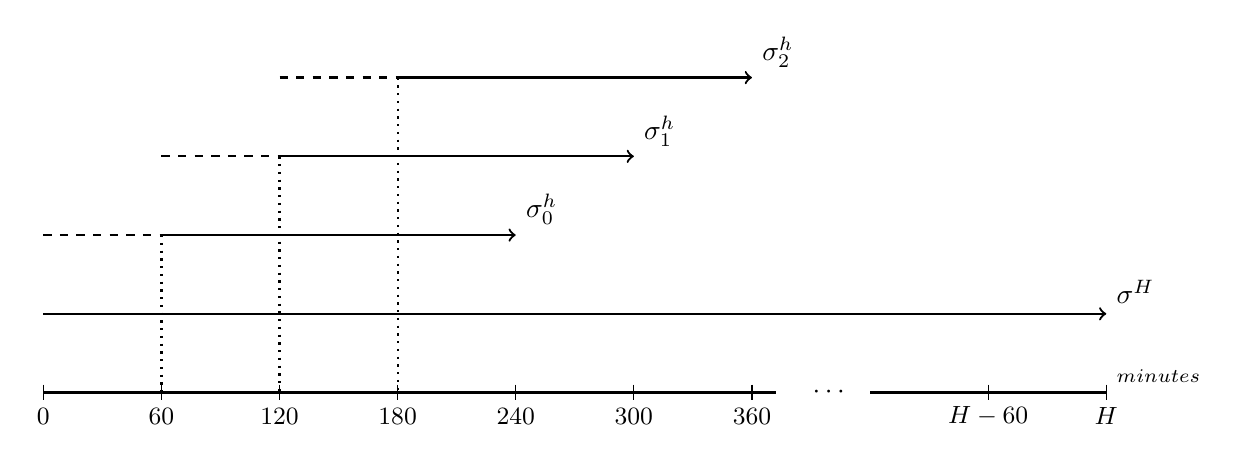
\begin{tikzpicture}[x=1.5cm]

      %%%%%%%%%%%% time division axis %%%%%%%%%%%%%%%
        \draw [thick] (-5, -2.5) -- (1.2, -2.5);
        \draw [thick] (2, -2.5) -- (4, -2.5)
        node[above right] {$\scriptstyle minutes$};
        \node [empty] at (1.65,-2.5) {$\cdots$};

        % Small tickmarks on the x axis
        \foreach \x/\l in {-5/0,-4/60,-3/120,-2/180,-1/240,0/300,1/360,3/{$H-60$},4/$H$} {
          \draw (\x, -2.4) -- (\x, -2.6);
          \node [empty] at (\x,-2.8) {\small \l};
          % \ifthenelse{\NOT -1 = \x \AND \NOT 0 = \x}{
          % \node [empty] at (\x,-2.8) {\small \l};}{
          % \ifthenelse{-1 = \x }{
          % \node [empty] at (\x-0.3,-2.8) {\small \l};}{
          % \node [empty] at (\x+0.4,-2.8) {\small \l};
          % }
          % }
        }

      %%%%%%%%%%%% first strategy %%%%%%%%%%%%%%%%%%%
      
      \draw [thick,->] (-5, -1.5) -- (4, -1.5)  node[above right]
      {$\sigma^H$};

      \draw [thick,dashed,-] (-5, -0.5) -- (-4, -0.5); % node {\textbullet};
      \draw [thick,->] (-4, -0.5) -- (-1, -0.5)  node[above
      right] {$\sigma^h_0$}; 
      %\useStrategy{-5}{-0.5}{-5}{-2.5};
      \draw [thick,dashed,-] (-4, 0.5) -- (-3, 0.5);
      \draw [thick,->] (-3, 0.5) -- (0, 0.5)  node[above
      right] {$\sigma^h_1$}; 
      \useStrategy{-4}{-0.5}{-4}{-2.5};
      \draw [thick,dashed,-] (-3, 1.5) -- (-2, 1.5);
      \draw [thick,->] (-2, 1.5) -- (1, 1.5)  node[above right] {$\sigma^h_2$};
      \useStrategy{-3}{0.5}{-3}{-2.5};
      \useStrategy{-2}{1.5}{-2}{-2.5};
    \end{tikzpicture}
  }
  \caption{Online Strategy Synthesis for $n$ \emph{cells}, a horizon
    $H$ of 1 day and controlling every 60 min. Short horizon $h$ of
    180 minutes.  For $n$ \emph{cells} for the offline controllers
    $\sigma^H$ and online controller $\sigma^h$ there are $2^{3n}$
    vs.\ $2^{720n}$ decisions.  }
  \label{fig:onlinestrategysynthesis}
\end{figure}




\begin{figure}[b]
  \centering
  \scalebox{0.8}{
    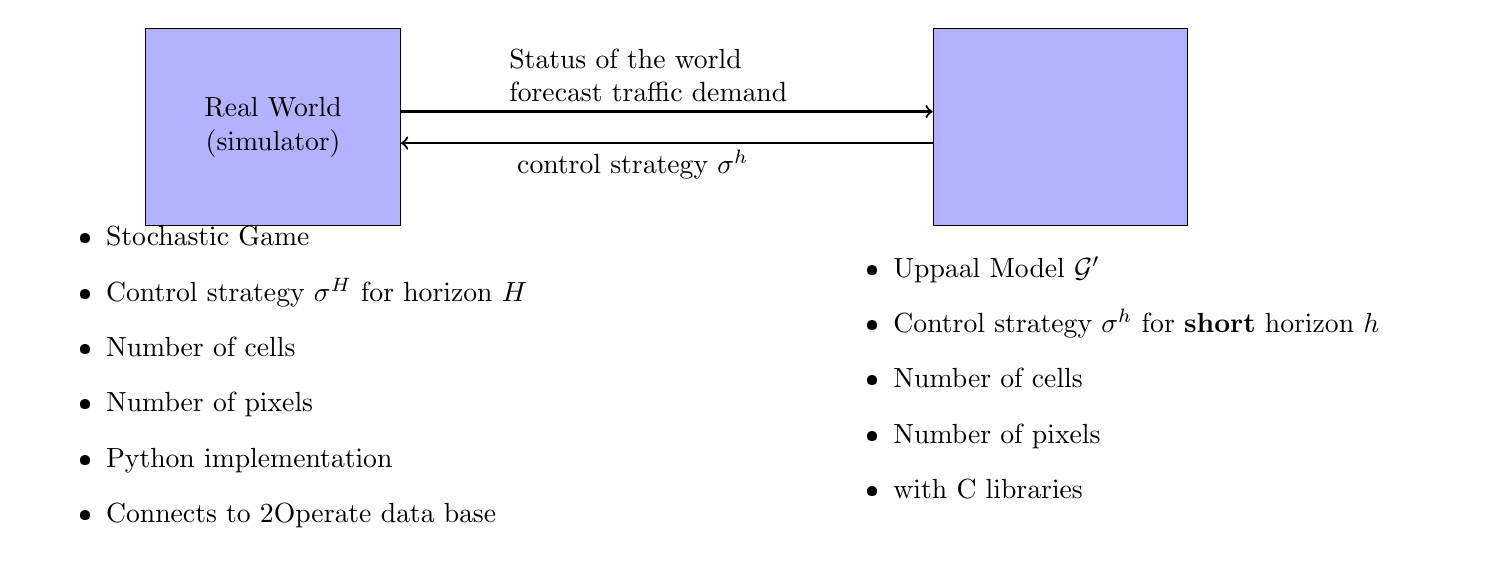
\begin{tikzpicture}
      \node (uppaal) at (10,0) [tool] {\stratego{}};
      \node (world) at (0,0) [tool] {Real World \\ (simulator)};

      \node (worlddes) at (1,-3) [empty] {{\parbox{8.0cm}{
            \flushleft
            \begin{itemize}
            \item
              Stochastic Game $\G$
            \item
              Control strategy $\sigma^H$ for horizon $H$
            \item
              Number of cells $\nrCells$
            \item
              Number of pixels $\nrPixels$
            \item
              {Python implementation}
            \item
              Connects to 2Operate data base
            \end{itemize}
          }}};

      \node (uppaaldes) at (11,-3) [empty] {{\parbox{8.0cm}{
            \flushleft
            \begin{itemize}
            \item
              Uppaal Model $\mathcal{G}'$
            \item
              Control strategy $\sigma^h$ for {\bf short} horizon $h$
            \item
              Number of cells $\nrCells$
            \item
              Number of pixels $\nrPixels$
            \item
              \stratego{} with C libraries
            \end{itemize}
          }}};
      
      
      \path[->,thick,black,draw,transform canvas={yshift=2mm}]
      (world) 
      edge node [above,pos=0.5] {\parbox{4.0cm}{\flushleft
          Status of the world \\ forecast traffic demand}}         
      (uppaal);
      \path[->,thick,black,draw,transform canvas={yshift=-2mm}]
      (uppaal) 
      edge node [below,pos=0.5,yshift=4mm, xshift=1mm] 
      {\parbox{4.0cm}{\flushleft
          control strategy $\sigma^h$}}         
      (world);
    \end{tikzpicture}
  }

  \caption{System Architecture}
  \label{fig:system}
\end{figure}

\subsection{Distributed Online Synthesis}

In this project we aim to control large scenarios with hundreds of
cells and millions of pixels. Therefore, directly applying online
strategy synthesis is not scalable. To overcome this difficulty, we
apply Distributed Online Synthesis as
in~\cite{DBLP:conf/tacas/LarsenMMST16}. Given a geographical area with
hundreds of cells, we partition it to sub areas which contain at most 8
cells. Then we can compute a online strategy for every partition and
then merge the strategies to control the full network.


\subsection{Methodology}

The real world consists of a number of base stations, cells, pixels,
frequency layers, etc.\ Where the goal is to provide a
\emph{controller} that powers ON or OFF cells to save energy. There
exist a number of tools which can be used to simulate the behavior of
mobile networks.
%

Figure~\ref{fig:system} illustrates our methodology. The real world
(or a simulation) require a control or a \emph{strategy} $\sigma^H$
for minimizing energy consumption for a long horizon $H$ e.g.\ 3
months. Since the number of choices for the controller grow
exponentially on the horizon $H$, computing a ``global'' strategy
$\sigma^H$ is not possible. Instead we periodically monitor the system
and compute a near-optimal strategy $\sigma^h$ for a short horizon
e.g.\ 3 hours. In this work we will use \stratego{} to compute online
strategies $\sigma^h$.







%%% Local Variables:
%%% mode: latex
%%% TeX-master: "main"
%%% End:
